\documentclass{article}
\usepackage[utf8]{inputenc}
\usepackage{geometry}
\usepackage{mathtools}
\usepackage{listings}
\usepackage{tikz}
\usetikzlibrary{arrows}
\lstset{language=Python} %declare python as language
\DeclarePairedDelimiter{\ceil}{\lceil}{\rceil}

\setcounter{totalnumber}{100}

\title{L05 \- Constraint Satisfaction}
\author{William Mak}
\date{January 05 2015}

\begin{document}

\maketitle
Restrictions on variables, Set of variables that represent your problem.\\
ex. Quantities in chemical reaction. Time/Schedule for operation.\\
\begin{enumerate}
	\item Set of variables $X_i$
	\item each variable has a domain $d_i$
	\item Goal test $\to$ checks for a solution.
\end{enumerate}

Assign colours such that no two adjacent countries share a colour\\
\section{Constraint Graph}
\textbf{Variables} \- Colour at each country\\
\textbf{Domain} \- $\{R, G, C, Y\}$
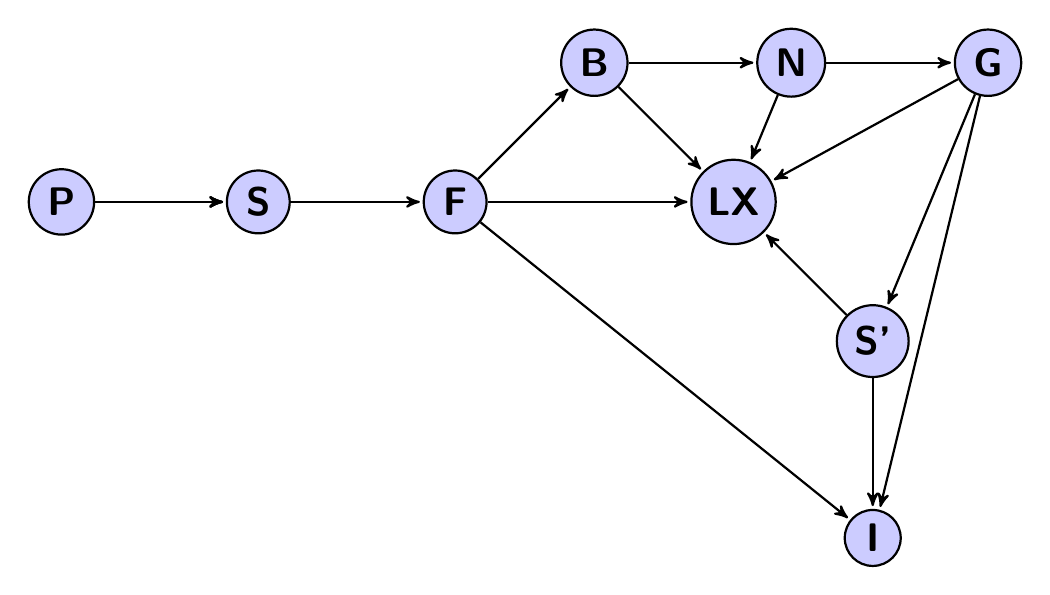
\begin{tikzpicture}[->,>=stealth',shorten >=1pt,auto,node distance=2.5cm,
  thick,main node/.style={circle,fill=blue!20,draw,font=\sffamily\Large\bfseries}]

  \node[main node] (P) {P};
  \node[main node] (S) [right of=P] {S};
  \node[main node] (F) [right of=S] {F};
  \node[main node] (B) [above right of=F] {B};
  \node[main node] (LX) [below right of=B] {LX};
  \node[main node] (N) [right of=B] {N};
  \node[main node] (S') [below right of=LX] {S'};
  \node[main node] (G) [right of=N] {G};
  \node[main node] (I) [below of=S'] {I};

  \path[every node/.style={font=\sffamily\small}]
    (P) edge node [] {} (S)
    (P) edge node [] {} (S)
    (S) edge node [] {} (F)
    (F) edge node [] {} (B)
    (F) edge node [] {} (LX)
    (B) edge node [] {} (LX)
    (N) edge node [] {} (LX)
    (S') edge node [] {} (LX)
    (G) edge node [] {} (LX)
    (S') edge node [] {} (I)
    (G) edge node [] {} (I)
    (F) edge node [] {} (I)
    (B) edge node [] {} (N)
    (N) edge node [] {} (G)
    (G) edge node [] {} (S')
    (P) edge node [] {} (S);
\end{tikzpicture}
\subsection{Using Search??}
\begin{enumerate}
	\item Types of \textbf{CSPs} -> which are we solving here?
	\item CSPs with continuous (Real valued variables)
	\item Discrete variables, finite -> graph colouring infinite -> schedulingg
\end{enumerate}
Don't use BFS. rather use DFS or in constraint graphs \textbf{"Backtracking Search"}\\
Choose variables from a root in some order.\\
Choose another variable.\\
If we come to a solution then we're done. But if there aren't any more possible 
nodes (Because of our constraints). Then go back up.
\subsection{Sudoku}
\textbf{Variables} \- $9 \times 9 = 81$ variables\\
\textbf{Constraint} \- sudoku.\\
Search has \textbf{A LOT of constraints!}\\
Allow search to break \underline{a few} constraints and then pay a penalty: 
$\sum_{Broken Constraints} W_i > {Total}$ Backtrack if the penalty surpasses 
some limit


\end{document}
